

\section*{4.2 利用者の管理とアクセス制御システムの整備}
% 独立した運用を行うためには利用者の管理とアクセス制御システムの整備が必要である.
% 既存の滞在ウォッチは単独コミュニティでのみの運用を前提としており開発者と管理者が同一であった.
% また利用者の権限に関する情報とそれに基づいたWebページログインの仕組みが存在せず,在室情報はプライバシに関わるものだが誰でも閲覧可能な状態であった.
% しかし複数コミュニティ間で運用を行う場合,コミュニティの数が増えるに連れてシステム開発者の利用者管理の負担が大きくなり運用するのは難しくなる.
% これを解決するには各コミュニティごとに管理者を作り,各コミュニティで独立した運用を行う必要がある.
% 各コミュニティごとに管理者が存在すればコミュニティの利用者の管理を全て行う必要がないため開発者の負担が軽減される.

% そこでGoogleアカウントを用いた利用者の認証機能を実装した.
% Googleアカウントを用いた認証のみでは,アカウント自体に滞在ウォッチに関する権限情報がないため利用者の識別はできない.
% そのため利用者の権限情報とアカウントを滞在ウォッチデータベースの利用者情報と紐づけている.
% これによりアカウントでログインしている利用者が管理者であるかの識別が可能である.

% また管理者が利用者の登録を行える仕組みを作成した.
% 利用者はシステム上にログインし,管理者にログインを行ったアカウントを報告する.
% 管理者が図2に示すWebページの利用者登録画面からそれを登録すると滞在ウォッチデータベースに利用者情報とGoogleアカウントが登録される.
% 利用者がログインした上でWebページを閲覧する際にWebページ側から利用者のアカウント情報を滞在ウォッチAPIサーバに送る.
% その後データベースにそのアカウントが登録されているかを確認する.
% 登録されている場合はWebページに対してその利用者の在室情報の閲覧の許可を与える.
% 仮に外部のものがGoogleアカウントを使ってログインしたとしてもデータベースにそのアカウントが登録されていないため在室情報の閲覧は不可能である.
% これにより適切な範囲での在室情報を扱うことが可能である.




独立した運用を行うためには利用者の管理とアクセス制御システムの整備が必要である.
既存の滞在ウォッチは単独コミュニティでのみの運用を前提としており開発者と管理者が同一であった.Web上からユーザの登録をするシステムが存在せずデータベースに対して直接変更を行うSQLを発行していた.
また利用者の権限に関する情報とそれに基づいたWebページログインの仕組みが存在せず,在室情報はプライバシに関わるものだが誰でも閲覧可能な状態であった.
しかし複数コミュニティ間で運用を行う場合,コミュニティの数が増えるに連れてシステム開発者の利用者管理の負担が大きくなり運用するのは難しくなる.
これを解決するには各コミュニティごとに管理者を作り,各コミュニティで独立した運用を行う必要がある.
各コミュニティごとに管理者が存在すればコミュニティの利用者の管理を全て行う必要がないため開発者の負担が軽減される.

そこでFirebase Authenticationを使ったGoogleプロバイダーによるOAuth認証を実装した.
OAuth (Open Authorization)は、ユーザーがサービスプロバイダー(例えばGoogle,FaceBookなど)に対して,別のサービスにアクセスするための権限を与えるためのオープンスタンダードの認証プロトコルである.
OAuth以外の認証方式としてBasic認証などがある.Basic認証はユーザ名とパスワードをベーシック認証ヘッダーに埋め込んで送信する方式である.この方式はセキュリティ上の問題が存在する.パスワードが暗号化されていないため,パスワードが盗まれる危険がある.また,Basic認証はバックエンド側でユーザ名とパスワードを保存する必要があり,管理を行うにはパスワードのハッシュ化など適切な処理を施す必要がある.
それと比較してOAuth認証では,ユーザのアカウント情報を第三者にアプリケーションに渡さずにアクセス権を付与できるため,セキュリティ上の利点がある.
OAuth認証では,アクセス権を持つアプリケーションにのみ有効で,期限切れになると,使用できなくなる.これにより,アクセス権を付与したアプリケーションが不正にアクセスするのを防止できる.
これらの理由により,OAtuh認証を採用した.

OAuthプロバイダーにはApple,FaceBookなど複数の選択肢がある中でGoogleを採用した.Googleアカウントは世界中で広く利用されており,多くの人がアカウントを持っているおり,多数の利用者に対応可能である.
Googleアカウントを用いたOAuth認証は,Googleアカウントを使って,サービスプロバイダー(Google)に対して,利用者が滞在ウォッチシステムにアクセスするための権限を与える.利用者はGoogleアカウントにログインし,Googleが提供するOAuth認証プロセスを通じて,滞在ウォッチシステムにアクセスできる.
OAuth認証により,利用者は自分のGoogleアカウントの情報(パスワードなど)を滞在ウォッチシステムに入力をせずに,安全にアクセスできる.
しかしGoogleアカウントによるOAuth認証だけでは意図しない外部のユーザのアクセスを防ぐことはできない.なぜならGoogleアカウントを持っているユーザなら誰でも認証を行えるためである.
そこでGoogleアカウントによるOAuth認証に加えて滞在ウォッチサーバ側で独自のユーザ認証を行った.具体的には滞在ウォッチ管理者が登録したユーザのみを認証するというものである.滞在ウォッチサーバのデータベースにはGoogleのアカウントのユーザ名であるメールアドレスが保存してある.この保存されたメールアドレスは滞在ウォッチの管理が登録したものであるため,メールアドレスが存在する場合は管理者の許可ある正規のユーザと判別が可能である.

以下で具体的なフローを説明する
まず初めに利用者は管理者に対してGoogleアカウントを報告する.
報告後管理者がWebの管理者ページのユーザ登録画面からGoogleアカウントを登録する.

ユーザには2種類のパターンが想定される.まず1つ目はBLEビーコンが既に登録済みのユーザ場合である.図〇〇に示す.
\begin{figure}[tbh]
  \centering
  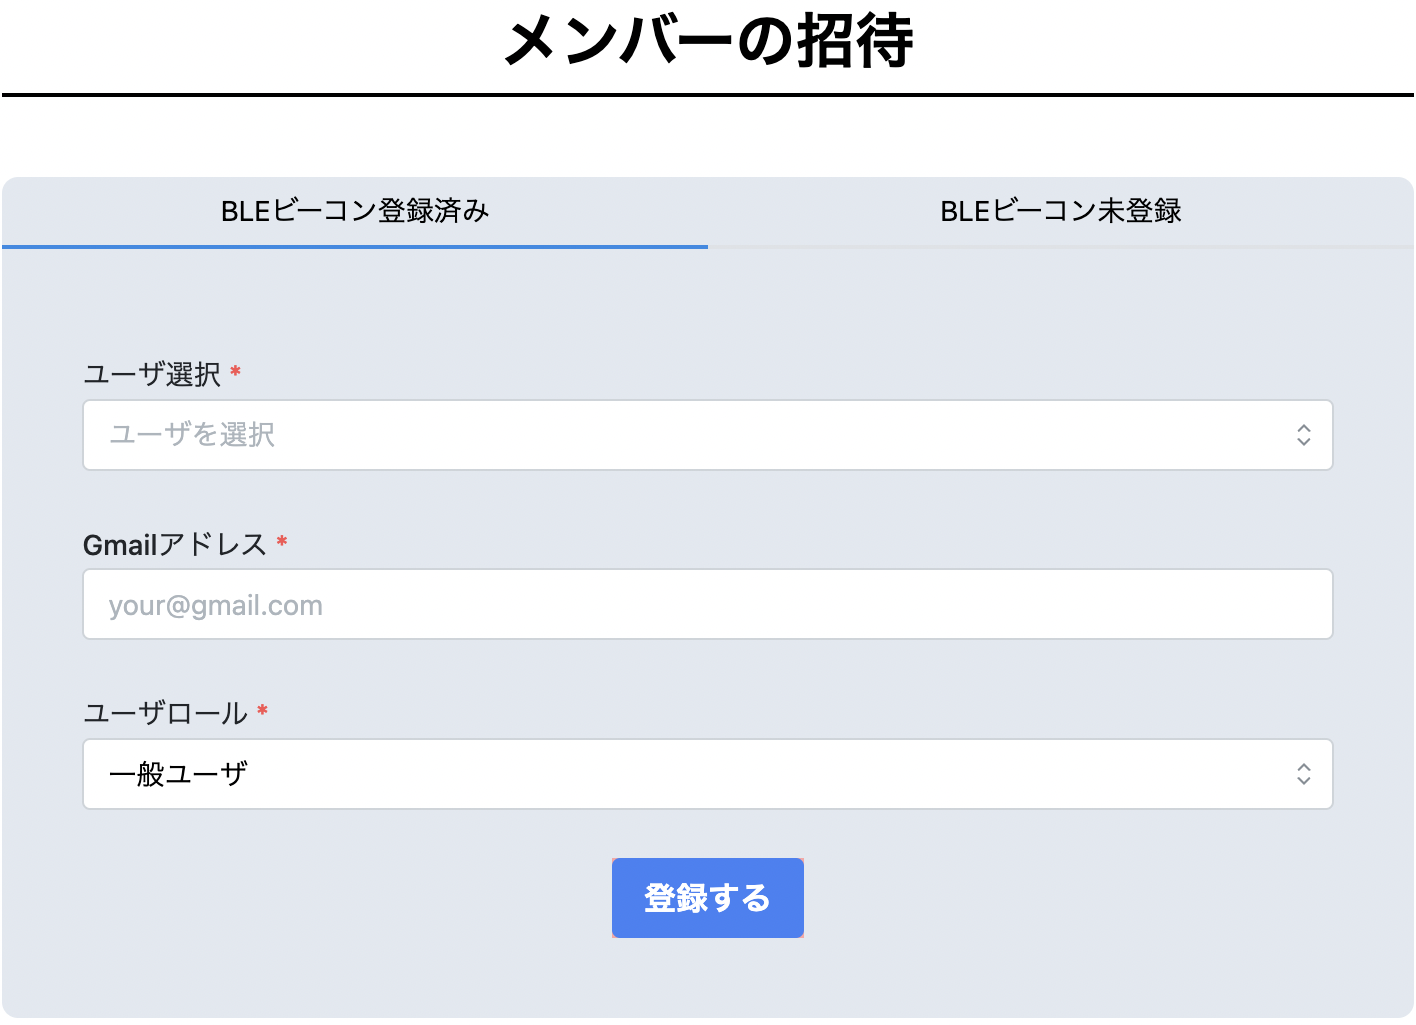
\includegraphics[width=16cm]{image/registerBLE.png}
  \caption{BLEビーコン登録済み}
  \label{multipleBPM}
\end{figure}
これは以前から滞在ウォッチユーザとして登録がされておりビーコンに関する情報とユーザ情報が既に存在しておりGoogleアカウントの情報とユーザロールのみがないユーザを想定している.
ユーザネームはデータベースに存在しているためバックエンドからデータを取得できる.
取得したデータをユーザが選択できるようにセレクトボックスを使用した.
ユーザロールのところでユーザの権限レベルの指定ができる.
一般ユーザと管理者ユーザの2つがあり,一般ユーザは滞在ウォッチの情報在室情報の閲覧などを行え,管理者ユーザはユーザの登録を行える.
登録されるとデータベースに存在するユーザにメールアドレスが紐づき,サーバ側は対象のメールアドレスに対して登録完了のメールを送信する.メールアドレスに対して通知を行うのはユーザがいつ登録が完了したのか気づけるようにするためである.
2つ目に想定されるのがBLEビーコンが登録されていない新規ユーザである.対象ユーザは4.3章で説明するスマホビーコンを使用する新規ユーザである.新規ユーザにはユーザネームがないため管理者はユーザネームを入力する必要がある.その他は1つ目と同じように入力して登録ボタンを押しサーバに対してリクエストを送信する.
1つめとの違いサーバ側は新規のUUIDの生成を行う.これによりGoogleアカウントを用いてスマホビーコンユーザの初期登録の際に生成されたUUIDを返すことができる.



\begin{figure}[tbh]
  \centering
  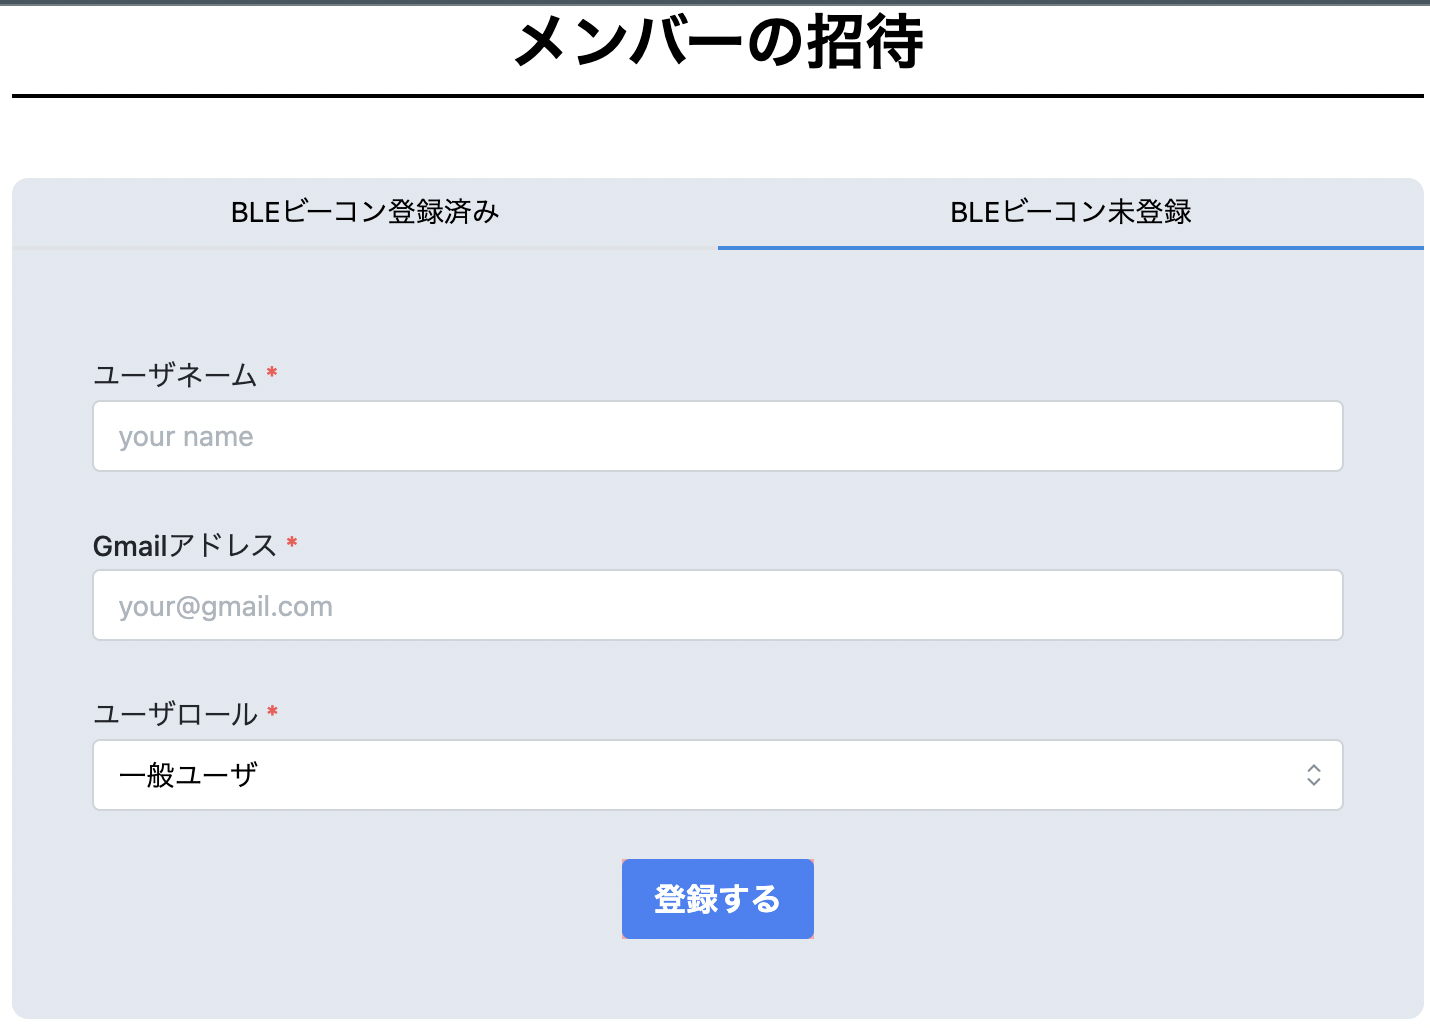
\includegraphics[width=16cm]{image/registerNotBLE.png}
  \caption{BLEビーコン登録済み}
  \label{multipleBPM}
\end{figure}



次にユーザ側に戻る
Fireabase Authで認証が成功するとJWT(JSON Web TOken)トークンが発行される.Firebase AuthのJWTトークン はFirebase Authが認証済みのユーザーを確認するために使用するトークンである.
JWTトークンは,JSON形式の文字列では発行者,トークンの有効期限,トークンの使用目的,サブジェクトが含まれておりユーザを一意に識別可能である.
JWTトークンは,フロントエンドから滞在ウォッチのバックエンドに送信される.
滞在ウォッチのバックエンドはFirebase AuthのAPIを使用して,JWTトークンの検証を行い,トークンが有効であるか確認する.有効なJWTトークンであった場合,アプリケーションのバックエンドは,そのトークンに含まれる情報を使用して,Firabase Authが認証済みであることを確認する.認証済みであった場合は次にメールアドレス情報を確認する.
データベースにメールアドレスが存在する場合フロントエンドに対してアクセスの許可を行うResponse Code 200を返す.

このプロセスによって不正なユーザの在室情報の閲覧を防いでいる.よって適切な範囲での在室情報の共有が可能である.






